\documentclass[11pt]{article}
% ===========================================================================
%  Shared preamble for all MPM2D worksheets — input right after \documentclass.
%  (Files beginning with "_" are skipped by mpm2d-worksheet-publish.mjs.)
% ===========================================================================
\usepackage[letterpaper,top=2.2cm,bottom=1.9cm,left=1.6cm,right=1.6cm,headheight=28pt,footskip=24pt]{geometry}
\usepackage{amsmath,amssymb}
\usepackage{cancel}
\usepackage[T1]{fontenc}
\usepackage[utf8]{inputenc}
\usepackage{lmodern}
\usepackage{xcolor}
\usepackage[most]{tcolorbox}
\usepackage{enumitem}
\usepackage{multicol}
\usepackage{fancyhdr}
\usepackage{tikz}
\usetikzlibrary{calc}
\usepackage{pgfplots}
\pgfplotsset{compat=1.18}

\definecolor{exblue}{HTML}{4A90E2}
\definecolor{exbg}{HTML}{E6F3FF}
\definecolor{qorange}{HTML}{E69138}
\definecolor{qbg}{HTML}{FFF7CC}
\definecolor{keygray}{HTML}{475569}
\definecolor{keybg}{HTML}{F1F5F9}
\definecolor{iagreen}{HTML}{14653B}
\definecolor{titleblue}{HTML}{1D4ED8}
% Rotating palette so each worked example gets its own colour.
\definecolor{ex0}{HTML}{2563A0}\definecolor{ex1}{HTML}{3B7D3B}\definecolor{ex2}{HTML}{8A5A00}
\definecolor{ex3}{HTML}{A3327A}\definecolor{ex4}{HTML}{6D28A3}\definecolor{ex5}{HTML}{B08900}
\definecolor{ex6}{HTML}{0E7490}\definecolor{ex7}{HTML}{9A3412}\definecolor{ex8}{HTML}{15803D}

\pagestyle{fancy}
\fancyhf{}
\fancyhead[L]{\footnotesize NAME: \underline{\hspace{3.4cm}}}
\fancyhead[C]{\textbf{Integration Academy}\\[-2pt]{\scriptsize Math Simplified \textperiodcentered{} Success Amplified}}
\fancyhead[R]{\footnotesize MPM2D}
\fancyfoot[L]{\scriptsize dr.merie@IntegrationAcademy.ca}
\fancyfoot[C]{\scriptsize\thepage}
\fancyfoot[R]{\scriptsize IntegrationAcademy.ca}
\renewcommand{\headrulewidth}{1.2pt}
\renewcommand{\footrulewidth}{0.4pt}
\setlength{\parindent}{0pt}
\setlength{\parskip}{4pt}

% Examples are NOT breakable, so each example + its solution stays on one page.
\newtcolorbox{example}[2]{colframe=#1,colback=#1!7,coltitle=white,colbacktitle=#1,fonttitle=\bfseries,title={#2},arc=3pt,boxrule=1pt}
\newtcolorbox{qbox}[1]{colframe=qorange,colback=qbg,coltitle=white,colbacktitle=qorange,fonttitle=\bfseries,title={#1},arc=3pt,breakable,boxrule=1pt}
\newtcolorbox{keybox}{colframe=keygray,colback=keybg,coltitle=white,colbacktitle=keygray,fonttitle=\bfseries,title={$\checkmark$\ Answer Key},arc=3pt,breakable,boxrule=1pt}
\newtcolorbox{recapbox}{colframe=keygray,colback=keybg,coltitle=white,colbacktitle=keygray,fonttitle=\bfseries,title={Question Recap},arc=3pt,breakable,boxrule=1pt}
\newtcolorbox{ideabox}{colframe=titleblue,colback=titleblue!6,coltitle=white,colbacktitle=titleblue,fonttitle=\bfseries,title={The Big Ideas},arc=3pt,breakable,boxrule=1.2pt}
\newtcolorbox{learnbox}{colframe=iagreen,colback=iagreen!5,coltitle=white,colbacktitle=iagreen,fonttitle=\bfseries,title={The Big Picture},arc=3pt,breakable,boxrule=1.2pt}
\newcommand{\lh}[1]{\par\smallskip{\bfseries\color{iagreen}#1}\par\nobreak\smallskip}

\newcommand{\soln}{\par\smallskip\textit{\textbf{Solution.}}\ }
\newcommand{\workspace}[1]{\par\vspace{3pt}\fcolorbox{black!30}{white}{\begin{minipage}[t][#1][t]{\dimexpr\linewidth-2\fboxsep\relax}\ \end{minipage}}\par}
\newcommand{\sech}[1]{\par\vspace{8pt}{\Large\bfseries\color{iagreen}#1}\par\nobreak\vspace{2pt}{\color{black!20}\hrule height1pt}\vspace{6pt}}

% A compact coordinate plot sized for an example box: \eplot{xmin}{xmax}{ymin}{ymax}{body}
\newcommand{\eplot}[5]{\begin{center}\begin{tikzpicture}
\begin{axis}[width=6.8cm,height=4.4cm,axis lines=middle,xlabel={\tiny$x$},ylabel={\tiny$y$},
grid=both,grid style={gray!16},xmin=#1,xmax=#2,ymin=#3,ymax=#4,
xtick distance=2,ytick distance=2,tick label style={font=\tiny},axis line style={-},samples=120]
#5
\end{axis}\end{tikzpicture}\end{center}}

% A sine-curve plot (degrees on x, 0..360): \splot{ymin}{ymax}{body}
\newcommand{\splot}[3]{\begin{center}\begin{tikzpicture}
\begin{axis}[width=8.6cm,height=4.6cm,axis lines=middle,xlabel={\tiny$x\,(^\circ)$},ylabel={\tiny$y$},
grid=both,grid style={gray!16},xmin=0,xmax=360,ymin=#1,ymax=#2,
xtick distance=90,ytick distance=1,tick label style={font=\tiny},axis line style={-},samples=180]
#3
\end{axis}\end{tikzpicture}\end{center}}

% A small coordinate plot: \plot{xmin}{xmax}{ymin}{ymax}{body}
\newcommand{\plot}[5]{\begin{center}\begin{tikzpicture}
\begin{axis}[width=8.4cm,height=6cm,axis lines=middle,xlabel={\scriptsize$x$},ylabel={\scriptsize$y$},
grid=both,grid style={gray!16},xmin=#1,xmax=#2,ymin=#3,ymax=#4,
xtick distance=2,ytick distance=2,tick label style={font=\tiny},axis line style={-}]
#5
\end{axis}\end{tikzpicture}\end{center}}

% Right triangle (angle theta at bottom-left, right angle at bottom-right):
%   \rtri{drawBase}{drawHeight}{oppLabel}{adjLabel}{hypLabel}
\newcommand{\rtri}[5]{\begin{center}\begin{tikzpicture}[scale=0.85]
\coordinate (A) at (0,0);\coordinate (B) at (#1,0);\coordinate (C) at (#1,#2);
\draw[thick,exblue] (A)--(B)--(C)--cycle;
\draw[black] ($(B)+(-0.32,0)$)--($(B)+(-0.32,0.32)$)--($(B)+(0,0.32)$);
\node[below] at ($(A)!0.5!(B)$){#4};
\node[right] at ($(B)!0.5!(C)$){#3};
\node[above left] at ($(A)!0.5!(C)$){#5};
\node at (0.7,0.22){$\theta$};
\end{tikzpicture}\end{center}}

% General (oblique) triangle with vertex labels and opposite-side labels:
%   \gtri{Alabel}{Blabel}{Clabel}{aSide}{bSide}{cSide}
\newcommand{\gtri}[6]{\begin{center}\begin{tikzpicture}[scale=0.85]
\coordinate (A) at (0,0);\coordinate (B) at (5,0);\coordinate (C) at (1.6,3);
\draw[thick,exblue] (A)--(B)--(C)--cycle;
\node[below left] at (A){#1};\node[below right] at (B){#2};\node[above] at (C){#3};
\node[below] at ($(A)!0.5!(B)$){#6};
\node[right] at ($(B)!0.5!(C)$){#4};
\node[left] at ($(A)!0.5!(C)$){#5};
\end{tikzpicture}\end{center}}

\fancyhead[R]{\footnotesize MCV4U \textperiodcentered{} 6.3}
\begin{document}

\begin{center}
{\LARGE\bfseries\color{titleblue}Worksheet 6.3 --- Cartesian Vectors in 2-D \& 3-D}\\[2pt]
{\small Grade 12 Calculus and Vectors (MCV4U) \textperiodcentered{} Unit 6: Geometry and Algebra of Vectors}
\end{center}

\begin{ideabox}
Component form $(a,b)$ or $(a,b,c)$; magnitude $\sqrt{a^2+b^2(+c^2)}$; operate componentwise; $\vec{AB}=B-A$; unit vector $\vec v/|\vec v|$.
\begin{itemize}[leftmargin=*,itemsep=2pt]
  \item $|(a,b)|=\sqrt{a^2+b^2}$, $|(a,b,c)|=\sqrt{a^2+b^2+c^2}$.
  \item Add/subtract/scale componentwise; $\vec{AB}=B-A$.
  \item Unit vector $\hat v=\vec v/|\vec v|$.
\end{itemize}
\end{ideabox}

\begin{learnbox}
\lh{Component form}A \textbf{Cartesian vector} is written by components, $\vec v=(x,y)$ or $(x,y,z)$, making calculations algebraic rather than geometric.
\lh{Magnitude}The magnitude is $\sqrt{x^2+y^2}$ in 2-D and $\sqrt{x^2+y^2+z^2}$ in 3-D — the distance formula in vector form.
\lh{Operations by component}Add, subtract, and scale vectors component by component; a unit vector is the vector divided by its magnitude.
\end{learnbox}

\sech{Worked Examples}

\begin{example}{ex0}{Example 1 --- Magnitude (2-D)}
Find $|(3,4)|$.\soln
\textbf{Step 1 (apply the 2-D magnitude formula):} $|(a,b)|=\sqrt{a^2+b^2}$.\\[3pt]
\textbf{Step 2 (substitute):} $\sqrt{3^2+4^2}=\sqrt{9+16}=\sqrt{25}$.\\[3pt]
\textbf{Conclusion:} $|(3,4)|=5$:\begin{center}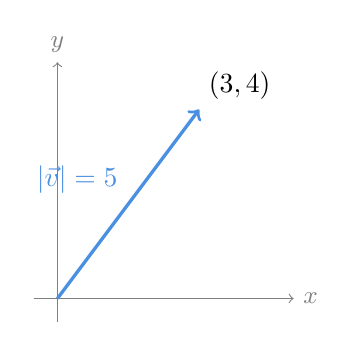
\begin{tikzpicture}[scale=0.6]\draw[->,gray](-0.5,0)--(5,0)node[right]{\small$x$};\draw[->,gray](0,-0.5)--(0,5)node[above]{\small$y$};\draw[->,very thick,exblue](0,0)--(3,4)node[midway,above left]{$|\vec v|=5$};\node at (3,4)[above right]{$(3,4)$};\end{tikzpicture}\end{center}
\end{example}

\begin{example}{ex1}{Example 2 --- Magnitude (3-D)}
Find $|(1,2,2)|$.\soln
\textbf{Step 1 (apply the 3-D magnitude formula):} $|(a,b,c)|=\sqrt{a^2+b^2+c^2}$.\\[3pt]
\textbf{Step 2 (substitute):} $\sqrt{1^2+2^2+2^2}=\sqrt{1+4+4}=\sqrt9$.\\[3pt]
\textbf{Conclusion:} $|(1,2,2)|=3$.
\end{example}

\begin{example}{ex2}{Example 3 --- Componentwise}
Compute $(2,3)+(1,-1)$ and $3(2,-1)$.\soln
\textbf{Step 1 (add component by component):} $(2+1,\,3+(-1))=(3,2)$.\\[3pt]
\textbf{Step 2 (scale each component by $3$):} $(3\cdot2,\,3\cdot(-1))=(6,-3)$.\\[3pt]
\textbf{Conclusion:} $(2,3)+(1,-1)=(3,2)$ and $3(2,-1)=(6,-3)$.
\end{example}

\begin{example}{ex3}{Example 4 --- Between points}
Find $\vec{AB}$ and $|\vec{AB}|$ for $A(1,2),B(4,6)$.\soln
\textbf{Step 1 (subtract $A$ from $B$, tail from tip):} $\vec{AB}=B-A=(4-1,\,6-2)=(3,4)$.\\[3pt]
\textbf{Step 2 (find the magnitude):} $|\vec{AB}|=\sqrt{3^2+4^2}=\sqrt{25}$.\\[3pt]
\textbf{Conclusion:} $\vec{AB}=(3,4)$, with length $5$.
\end{example}

\begin{example}{ex4}{Example 5 --- Unit vector}
Unit vector of $(3,4)$.\soln
\textbf{Step 1 (find the magnitude):} $|(3,4)|=\sqrt{9+16}=5$.\\[3pt]
\textbf{Step 2 (divide each component by the magnitude):} $\left(\dfrac35,\dfrac45\right)$.\\[3pt]
\textbf{Conclusion:} the unit vector is $\big(\tfrac35,\tfrac45\big)$.
\end{example}

\begin{example}{ex5}{Example 6 --- Magnitude (2-D)}
Find $|(6,8)|$.\soln
\textbf{Step 1 (apply the magnitude formula):} $\sqrt{6^2+8^2}=\sqrt{36+64}=\sqrt{100}$.\\[3pt]
\textbf{Conclusion:} $10$.
\end{example}

\begin{example}{ex6}{Example 7 --- Magnitude (3-D)}
Find $|(2,3,6)|$.\soln
\textbf{Step 1 (apply the 3-D magnitude formula):} $\sqrt{2^2+3^2+6^2}=\sqrt{4+9+36}=\sqrt{49}$.\\[3pt]
\textbf{Conclusion:} $7$.
\end{example}

\begin{example}{ex7}{Example 8 --- Componentwise}
Compute $(5,1)-(2,4)$.\soln
\textbf{Step 1 (subtract component by component):} $(5-2,\,1-4)$.\\[3pt]
\textbf{Conclusion:} $(3,-3)$.
\end{example}

\begin{example}{ex8}{Example 9 --- Between points}
Find $\vec{AB}$ for $A(2,1),B(5,5)$.\soln
\textbf{Step 1 (subtract $A$ from $B$):} $(5-2,\,5-1)$.\\[3pt]
\textbf{Conclusion:} $\vec{AB}=(3,4)$.
\end{example}

\clearpage
\sech{Your Turn --- Show Your Work}
For each question, show all steps clearly in the space provided.

\begin{qbox}{Question 1}
Find $|(6,8)|$.\workspace{2.4cm}
\end{qbox}

\begin{qbox}{Question 2}
Find $|(2,3,6)|$.\workspace{2.4cm}
\end{qbox}

\begin{qbox}{Question 3}
Compute $(5,1)-(2,4)$.\workspace{2.4cm}
\end{qbox}

\begin{qbox}{Question 4}
Find $\vec{AB}$ for $A(2,1),B(5,5)$.\workspace{2.4cm}
\end{qbox}

\begin{qbox}{Question 5}
Unit vector of $(6,8)$?\workspace{2.4cm}
\end{qbox}

\begin{qbox}{Question 6}
Find $|(5,12)|$.\workspace{2.4cm}
\end{qbox}

\begin{qbox}{Question 7}
Find $|(1,4,8)|$.\workspace{2.4cm}
\end{qbox}

\begin{qbox}{Question 8}
Compute $(3,2)+(4,-5)$.\workspace{2.4cm}
\end{qbox}

\begin{qbox}{Question 9}
Compute $2(3,-4)$.\workspace{2.4cm}
\end{qbox}

\begin{qbox}{Question 10}
Find $|\vec{AB}|$ for $A(0,0),B(8,6)$.\workspace{2.4cm}
\end{qbox}

\begin{qbox}{Question 11}
Unit vector of $(0,5)$?\workspace{2.4cm}
\end{qbox}

\begin{qbox}{Question 12}
Find $|(7,24)|$.\workspace{2.4cm}
\end{qbox}

\begin{qbox}{Question 13 --- Challenge}
Given $A(1,2,3)$ and $B(4,6,15)$, find $\vec{AB}$ and $|\vec{AB}|$.\workspace{3cm}
\end{qbox}

\clearpage
\sech{Question Recap \& Answer Key}

\begin{recapbox}
\begin{multicols}{2}
\small
\begin{enumerate}[leftmargin=*,itemsep=3pt]
  \item Find $|(6,8)|$.
  \item Find $|(2,3,6)|$.
  \item Compute $(5,1)-(2,4)$.
  \item Find $\vec{AB}$ for $A(2,1),B(5,5)$.
  \item Unit vector of $(6,8)$?
  \item Find $|(5,12)|$.
  \item Find $|(1,4,8)|$.
  \item Compute $(3,2)+(4,-5)$.
  \item Compute $2(3,-4)$.
  \item Find $|\vec{AB}|$ for $A(0,0),B(8,6)$.
  \item Unit vector of $(0,5)$?
  \item Find $|(7,24)|$.
  \item Given $A(1,2,3)$ and $B(4,6,15)$, find $\vec{AB}$ and $|\vec{AB}|$.
\end{enumerate}
\end{multicols}
\end{recapbox}

\begin{keybox}
\begin{multicols}{2}
\small
\begin{enumerate}[leftmargin=*,itemsep=3pt]
  \item $10$
  \item $7$
  \item $(3,-3)$
  \item $(3,4)$
  \item $(\tfrac35,\tfrac45)$
  \item $13$
  \item $9$
  \item $(7,-3)$
  \item $(6,-8)$
  \item $10$
  \item $(0,1)$
  \item $25$
  \item $(3,4,12)$, $|\vec{AB}|=\sqrt{9+16+144}=13$
\end{enumerate}
\end{multicols}
\end{keybox}

\end{document}
